%%%%%%%%%%%%%%%%%%%%%%%%%%%%%%%%%%%%%%%%%%%%%%%%%%%
%% P3: Phenomenology of Particle Physics                         
%%
%% Author:  André Rubbia                   		 
%%
%% Figure 2.19 Illustration of Chadwick's experimental setup to study the production of secondary particles when $\alpha$ particles hit a beryllium target.
%%
%% This work is licensed under the Creative Commons Attribution 4.0 International License. 
%% To view a copy of this license, visit http://creativecommons.org/licenses/by/4.0/ or 
%% send a letter to Creative Commons, PO Box 1866, Mountain View, CA 94042, USA.
%%
%%
%%%%%%%%%%%%%%%%%%%%%%%%%%%%%%%%%%%%%%%%%%%%%%%%%%%

\documentclass[a4paper,10pt]{article}

\usepackage[T1]{fontenc}
\usepackage[utf8]{inputenc}
\usepackage{lmodern}
\usepackage[labelfont=bf]{caption}
\usepackage{upgreek}
\usepackage{amssymb}
\usepackage{amsmath}

\usepackage{tikz}
\usetikzlibrary{patterns}
\usetikzlibrary{decorations.pathmorphing}
\usetikzlibrary{decorations.markings}
\usetikzlibrary{arrows}
\usetikzlibrary{svg.path}
\usetikzlibrary{shapes}
\usetikzlibrary{arrows.meta}
% define the arrow style
\tikzset{
    arrow/.style={
        decoration={
            markings,
            mark=at position .5 with {
                \arrow[#1, scale=1.5]{latex}
            }
        },
        postaction={decorate},
    }
}
\tikzset{
    arrow flipped/.style={
        decoration={
            markings,
            mark=at position .5 with {
                \arrow[#1, scale=1.5]{latex reversed}
            }
        },
        postaction={decorate},
    }
}
\pgfkeys{/pgf/number format/.cd,1000 sep={}}

\usepackage{pgfplots}
\pgfplotsset{compat=1.17}
\usepgfplotslibrary{ternary}
\usepgfplotslibrary{fillbetween}
\usepgfplotslibrary{external}


\def\d{\mathrm{d}}

\begin{document}

%%%%%%%%%%%%%%%   FIGURE  %%%%%%%%%%%%%%%%%%%%%%%%%%%%%%
\begin{figure}[htb]
\begin{center}
\vspace{5mm}
    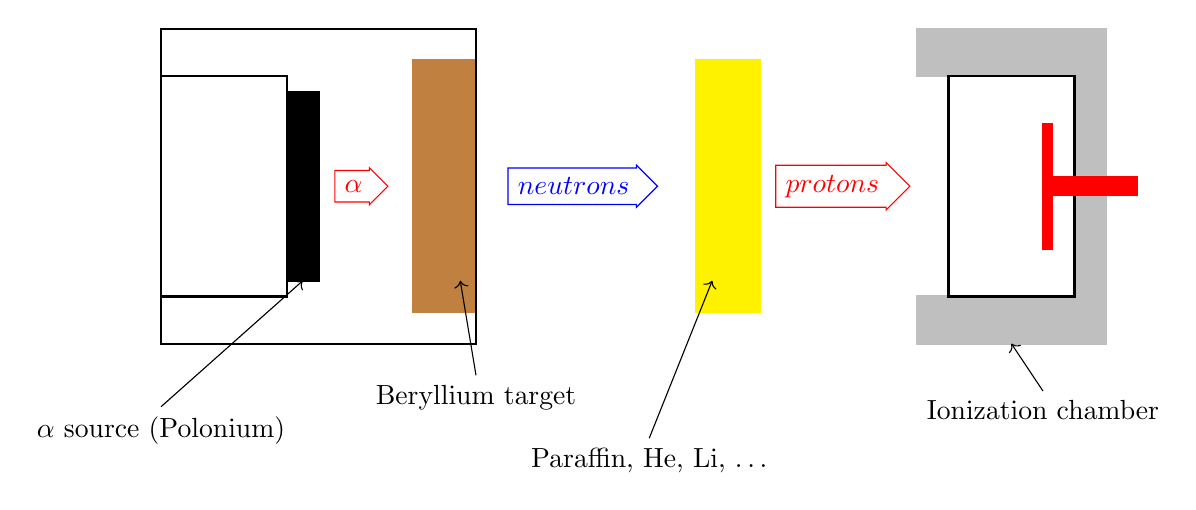
\begin{tikzpicture}[scale=4]
         \draw[thick] (0.,0.15) -- (0.4,0.15) -- (0.4,0.85) -- (0.0,0.85) -- cycle;
         \draw[thick,fill,color=black] (0.4,0.2) -- (0.5,0.2) -- (0.5,0.8) -- (0.4,0.8) -- cycle;
         \draw[thick,fill,color=brown] (0.8,0.1) -- (1,0.1) -- (1,0.9) -- (0.8,0.9) -- cycle;
         \draw[thick] (0,0) -- (1,0) -- (1,1) -- (0,1) -- cycle;
         \draw[<-] (0.45,0.2) -- (0,-0.2) node[below] {$\alpha$ source (Polonium)};
         \draw[<-] (0.95,0.2) -- (1.,-0.1) node[below] {Beryllium target};
 %
         \draw[thick,fill,color=yellow] (1.7,0.1) rectangle (1.9,0.9);
         \draw[<-] (1.75,0.2) -- (1.55,-0.3) node[below] {Paraffin, He, Li, $\ldots$};
%
  \begin{scope}[shift={(2.5,0)}]
        \draw[thick,fill,color=lightgray] (-0.1,0.15) -- (0.4,0.15) -- (0.4,0.) -- (-0.1,0.) -- cycle;
        \draw[thick,fill,color=lightgray] (-0.1,0.85) -- (0.4,0.85) -- (0.4,1) -- (-0.1,1) -- cycle;
        \draw[thick,fill,color=lightgray] (0.4,0) -- (0.5,0.0) -- (0.5,1) -- (0.4,1) -- cycle;
        \draw[thick] (0.,0.15) -- (0.4,0.15) -- (0.4,0.85) -- (0.0,0.85) -- cycle;
        \draw[fill, color=red] (0.3,0.3) rectangle (0.33,0.7);
        \draw[fill, color=red] (0.33,0.47) rectangle (0.6,0.53);
         \draw[<-] (0.2,0) -- (0.3,-0.15) node[below] {Ionization chamber};
 \end{scope}
 % particles
 \node[draw, color=blue, single arrow,
              minimum height=0.5, minimum width=0.2,
              single arrow head extend=1,
              anchor=west, rotate=0] at (1.1,0.5) {$neutrons$};
 \node[draw, color=red, single arrow,
              minimum height=0.5, minimum width=0.2,
              single arrow head extend=1,
              anchor=west, rotate=0] at (1.95,0.5) {$protons$};
 \node[draw, color=red, single arrow,
              minimum height=0.5, minimum width=0.2,
              single arrow head extend=1,
              anchor=west, rotate=0] at (0.55,0.5) {$\alpha$};
  \end{tikzpicture}
\caption{Illustration of Chadwick's experimental setup to study the production of secondary particles
when $\alpha$ particles hit a beryllium target.}
\end{center}
\end{figure}
%%%%%%%%%%%%%%%   END FIGURE  %%%%%%%%%%%%%%%%%%%%%%%%%%%%%%

\end{document}
